\documentclass[a4paper,12pt]{article}
\usepackage{graphicx}
\usepackage{hyperref}

\title{Project Execution Plan}
\author{Arshad Beg}
\date{\today}

\begin{document}

\maketitle

\section{Execution of the Project}
\label{app:proj_execution}

As our project aims to explore how large language models (LLMs) like ChatGPT-4, Qwen, or Claude can help with formal verification of C programs using Frama-C and SMT solvers, the execution proceeds as follows.

In the first month, we prepare a dataset of about 50 C programs, each with annotated requirements. For a more practical and complex set of programs, we are in contact with the developer team of Frama-C. Simultaneously, we set up the verification tools�Frama-C with WP and RTE plugins, plus solvers like Z3, CVC4, and CVC5�and ensure all components work together smoothly. We also design prompts to guide the LLMs in extracting requirements and generating annotations. By the end of this phase, we will have a solid dataset, a tested toolchain, and a prompt library.

\begin{figure}[ht]
    \centering
    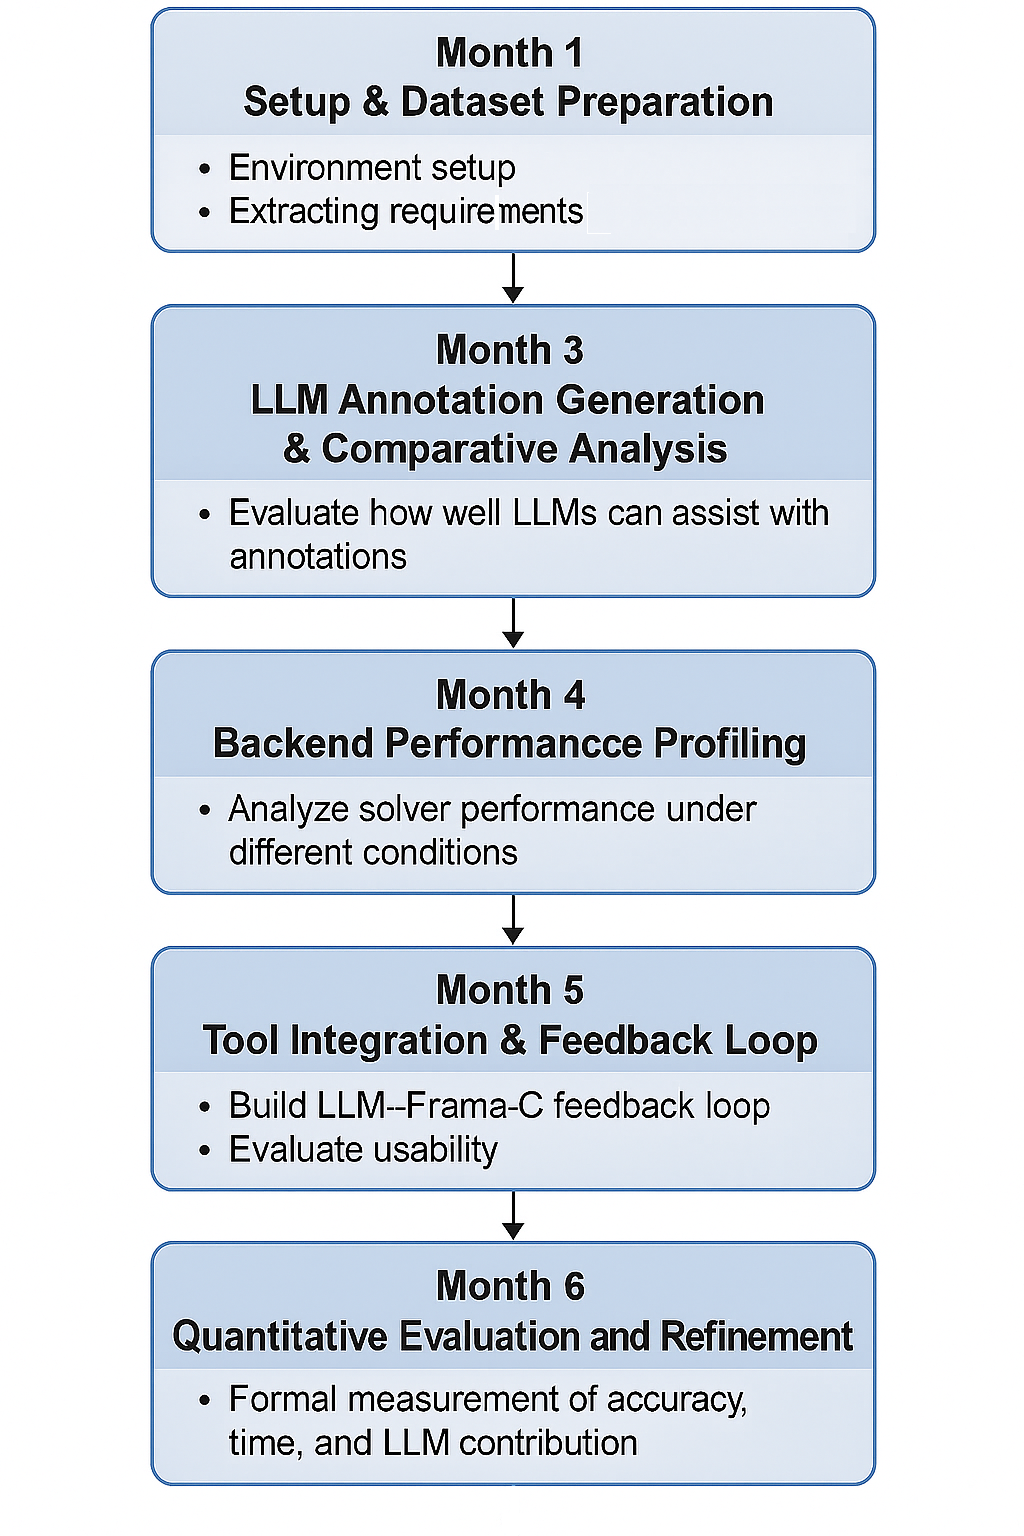
\includegraphics[width=7cm,height=10cm,keepaspectratio]{WorkPlan-NextSixMonths.png}
    \caption{Work Plan for Next Few Months}
    \label{fig:workplan}
\end{figure}

Next, we focus on extracting requirements from code using LLMs and checking their accuracy. These extractions are compared to gold-standard annotations or manual reviews to ensure quality. We then perform baseline verification using Frama-C and the RTE annotations with multiple solvers, to establish benchmarks of current verification performance and speed prior to introducing LLM-generated annotations.

In month three, LLMs are used to generate formal ACSL annotations, such as preconditions and assertions. These annotations are validated for syntax and semantics, followed by another round of verification. Comparing these results to the baseline helps us evaluate the value LLMs add to the annotation process. We produce a dataset containing code with LLM-generated annotations and a report analyzing their effectiveness.

The fourth month is dedicated to testing solvers. We run verification tasks on Z3, CVC4, and CVC5 to evaluate time, success rates, and output clarity. These insights help us refine our LLM prompts to generate annotations better suited to the solvers. The main outcomes are a performance comparison of solvers and improved prompt strategies.

In month five, we develop a semi-automated workflow. This system takes C code, generates annotations with LLMs, verifies them with Frama-C, and uses the results to enhance the prompts. We test the workflow on a new dataset to evaluate its practical utility. Outputs include a working prototype and an evaluation report on its accuracy and usability.

In month six, we define clear metrics such as annotation precision, verification success, solver runtime, and prompt efficiency. We then address bottlenecks found in the solvers or prompt design through iterative refinements. The goal is to improve the system�s accuracy and speed. This phase concludes with a metrics report and a refined verification framework.

Finally, in the seventh month, we integrate all components. We produce a comprehensive technical report and a paper describing our methodology, tools, datasets, experiments, and findings. A demo is also prepared to showcase the automated workflow verifying five new C programs�either live or as a recording.

\end{document}